\begin{frame}
\frametitle{Va chạm}
Xét hai vật có khối lượng \(m_1\) và \(m_2\) chuyển động với vận tốc \(v_1\) và \(v_2\). Tìm vận tốc sau va chạm \(v_1'\) và \(v_2'\) của chúng. Biết rằng va chạm là hoàn toàn đàn hồi.
\begin{figure}
    \centering
    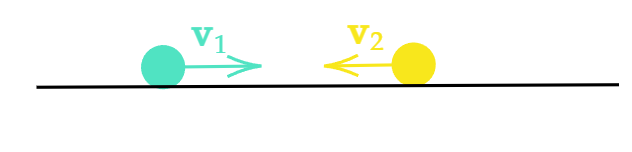
\includegraphics[width=0.4\textwidth]{Content/Figure/collision.png}
\end{figure}
\pause
\begin{columns}
\begin{column}{0.5\textwidth}
\scriptsize
Định luật bảo toàn động lượng:
\begin{equation*}
    m_1 v_1 - m_2 v_2 = m_1 v_1' - m_2 v_2'.
\end{equation*}
Định luật bảo toàn năng lượng:
\begin{equation*}
    \frac{m_1 v_1^2}{2} + \frac{m_2 v_2^2}{2} = \frac{m_1 {v_1'}^2}{2} + \frac{m_2 {v_2'}^2}{2}.
\end{equation*}
\normalsize
\end{column}
\begin{column}{0.5\textwidth}
Giải hệ phương trình trên ta được:
\begin{equation}
    \begin{aligned}
    v_1' = \frac{(m_1 - m_2)v_1 + 2m_2 v_2}{m_1 + m_2},\\
    v_2' = \frac{(m_2 - m_1)v_2 + 2m_1 v_1}{m_1 + m_2}.
    \end{aligned}
\end{equation}
\end{column}
\end{columns}
\end{frame}